\documentclass{article}

\usepackage[utf8]{inputenc}
\usepackage{amsthm}
\usepackage{amssymb}
\usepackage{amsfonts}
\usepackage[francais]{babel}
\usepackage{fancyvrb}
\usepackage{hyperref}
\usepackage{listings}
\usepackage{graphicx}
\usepackage{blindtext}
\usepackage{enumitem}


\title{Compte rendu TP3\\ Equations différentielles}

\begin{document}

\maketitle



\begin{enumerate}
\item
	\begin{enumerate}
	\item
  Dans cet exemple, la fonction f vaut -u.

	\item
  En calculant à la main, on trouve que f(t) vaut exp(-t).
En effet, si u' = -u, alors, u(t)'/u(t) = -1, en primitivant les deux expressions, on trouve: ln(u(t)) = -t. Ainsi, en appliquant l'exponentiel de chaque coté, on a: u(t) = exp(-t)

	\item
  Pour exprimer et tracer la fonction exp(-t), on code le programme suivant:

\begin{lstlisting}[basicstyle=\small]
import matplotlib.pyplot as plt
import numpy as np
import scipy as sp


def f(x):
    return sp.e**-x

x = np.arange(0, 2, 0.1)
plt.plot(x, f(x),'r-')
plt.grid('on')
plt.axis('equal')
plt.show()

\end{lstlisting}

	\end{enumerate}

\item La méthode d'Euler permet d'approximer la solution d'une equation diférentielle ordinaire. 
On calcule une suite d'approximations à l'aide de la formule 
$u_{k+1} = u_k + hf(t_k, u_k)$

Avec sur un intervalle [0,T], h = T/n
\begin{enumerate}
Calculons les n+1 termes de la suite  $(u_k)$
On défini les fonctions f(t,u) et u(x):

\begin{lstlisting}[basicstyle=\small]
def f(t,u):
	return -u

def u(x):
	return exp(-x)
\end{lstlisting}
On défini des listes, qu'on utilisera plus tard pour tracer les graphes;
X est la liste contenant les $t_k$ pour k allant de 0 à n \\
U est la liste contenant les n+1 premiers termes de la suite $(u_k)$ \\
Y contient les images par la fonction u(x) = exp(-x) \\

On a :
\begin{lstlisting}[basicstyle=\small]
T = 2.0
n=10
h = float (T)/n
X,U = [],[]
u0=1
x0=0

ui=u0
xi=x0

X.append(x0)
U.append(u0)

for i in range (0,n):
	xi = xi + h
	ui = ui + h*f(xi,ui)
	X.append(xi)
	U.append(ui)
print(X)
print(U)
\end{lstlisting}
Les n + 1 premiers termes de la suite $(u_k)$ sont avec ce code \\
U = [1, 0.8, 0.64, 0.512, 0.4096, 0.32768, 0.26214400000000004, \\ 0.20971520000000005, 0.16777216000000003, 0.13421772800000004,  \\ 0.10737418240000003]

\item 
On trace avec matplotlib la solution exacte u et les points ($t_k$,$u_k$)
\begin{center}
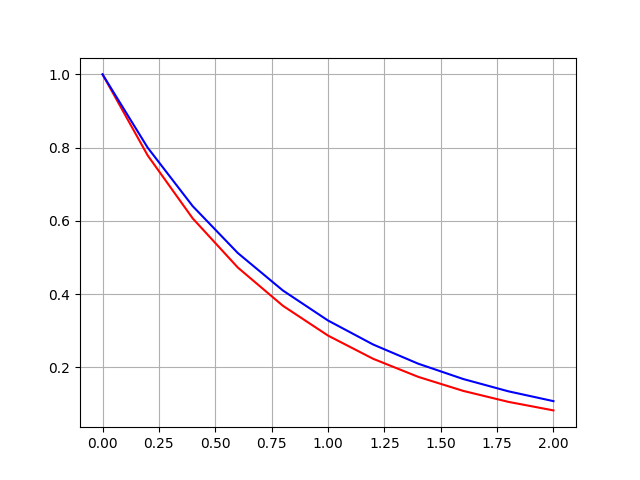
\includegraphics{exo2graph.png}
\end{center}

\end{enumerate}

\begin{enumerate}
\item
On définit la fonction euler: 
\begin{lstlisting}[basicstyle=\small]
def euler(f,u0,T,n):
 

  h = float (T)/n
  tt,uu = [],[]
  x0=0

  ui=u0
  xi=x0

  tt.append(x0)
  uu.append(u0)

  for i in range (x0,n):
	xi = xi + h
	ui = ui + h*f(xi,ui)
	tt.append(xi)
	uu.append(ui)
 
  return tt,uu 
\end{lstlisting}
ce programme prend en paramètre une fonction puis, elle liste les n+1 premiers termes qui sont solutions de l'équation différentielle en x = k* T/n
avec k allant de 0 à n.

\end{enumerate}

\begin{enumerate}
\item
	
	\item
	
Voici le programme permettant d'écrire la fonction de l'exemple 2 puis, d'appliquer la fonction euler :
\begin{lstlisting}[basicstyle=\small]
import matplotlib.pyplot as plt
from numpy import *
from math import *
from pylab import *
from methods import euler


def u(t,u):
	return exp(-t)

X,Y = [],[]
X,Y = euler(u,1,2,10)

print X,Y

\end{lstlisting}

    \item résolution des EDO à la main en pièce jointe(1)
Nous avons essayé de résoudre la 3e EDO à la main pour être sûr qu'elle était difficilement résolvable à la main
\begin{align*} 
u'(t) &= u^2(t) - t, & u(0) &= 1.0
\end{align*}
(voir pièce jointe 2)
\end{enumerate}
\item
\begin{enumerate}
\item
(voir pièce jointe 3)
\item
Avant de définir F, on définit un numpy array U, qui facilitera l'execution de la fonction Euler qui prendra le numpy array en argument
\begin{lstlisting}[basicstyle=\small]
import matplotlib.pyplot as plt
import numpy as np
from math import *
from pylab import *

def U(u,v):
	return np.array([u,v])

def F(t,U):
	return np.array([U[1],-U[0]])

\end{lstlisting}
\item
Au lieu de modifier la fonction euler, on a crée une 2e fonction noté "Euler". La fonction a la même structure que euler mais admet quelques changements:
\begin{lstlisting}[basicstyle=\small]

def Euler(F,U0,T,n):
	h = float (T)/n
	
	tt = np.linspace(0,T,n+1)
	suite = [U0]
	for i in range(0,n):
		U0 = U0 + h*F(h*i,U0)
		suite.append(U0)
	UU = np.asarray(suite)
	return tt,UU
\end{lstlisting}
La fonction np.linspace permet d'obtenir un tableau à une dimension allant d'une valeur de départ à une valeur de fin avec un nombre donné d'élément. La fonction remplace donc la boucle $for$ et le $"tt.append"$ présents dans l'autre fonction euler
La fonction np.asarray permet de convertir la liste "suite" en array noté "UU"
\item 
On essaie la fonction Euler pour $w = 1$ et $T = 4\pi$
\begin{lstlisting}[basicstyle=\small]
N=1000

tt,UU = Euler(F,U(1,0),4*np.pi,N)
x = np.linspace(0, 4*np.pi,100)
y=np.cos(x)
print tt,UU
\end{lstlisting}
En essayant différentes valeurs de N, on remarque que plus le N est grand, plus Euler approche la fonction (voir pieces jointes)
On trace ces graphes à l'aide des codes :
\begin{lstlisting}[basicstyle=\small]
plt.title('u en fonction du temps')
plt.plot(x, y, color = 'green')
plt.scatter(tt, [UU[i][0] for i in range(N+1)], color='red', marker='.')
plt.show()

plt.title('v en fonction du temps')
plt.plot(x, y2, color = 'green')
plt.scatter(tt, [UU[j][1] for j in range(N+1)], color='red', marker='.')
plt.show()

plt.title('v en fonction de u')
plt.plot(x, y3, color = 'green')
plt.scatter(tt, [UU[j][1] for j in range(N+1)], color='red', marker='.')
plt.show()
\end{lstlisting}
y2 est la dérivé de y, y vaut $cos(x)$ donc y2 = $-sin(x)$
y3 est le résultat de v en fonction de u, on a défini u et v en fonction du temps, on défini donc y3 = $- sin(arccos(x)$
Le 3e graphe admet toutefois une erreur, la coubre verte s'arrête, elle n'est défini que sur une petite fenêtre. Nous n'avons pas compris d'où venait l'erreur
\end{enumerate}
\end{document}
